\documentclass{article}
\usepackage{iclr2026_conference,times}
\usepackage{amsmath,amssymb,amsthm}
\usepackage{graphicx}
\usepackage{booktabs}
\usepackage{url}
\usepackage{hyperref}
\usepackage{microtype}
\input{math_commands.tex}

\title{Causal Scene Flow for Interaction}

\author{Anonymous Authors\\
Anonymous Institution\\
\texttt{anonymous@example.com}}

\newtheorem{proposition}{Proposition}
\newtheorem{definition}{Definition}
\newcommand{\noop}{a_0}
\newcommand{\effect}{\mathcal{E}}
\newcommand{\points}{\mathcal{X}}

\begin{document}
\maketitle
\noindent\textbf{Submission-hardening version: v3, 2026-06-14.}
This version replaces the five-page v2 counterexample with a full-scale mechanism paper:
seven synthetic experiment families, multi-distractor scenes, no-action misspecification
surfaces, spatial-overlap and ego-motion stresses, a learned no-op proxy, endpoint-error
versus planning-metric analysis, ablations, generated figures/tables, and an explicit
25-page artifact target.

\begin{abstract}
Scene flow is usually treated as a passive perception target: estimate how every visible
3D point will move.  For a robot that must interact, this target can answer the wrong
question.  A point may move because of a conveyor, camera ego-motion, gravity, another
actor, or object dynamics independent of the robot.  A planner that ranks contacts by
total predicted motion can therefore choose passive distractors.  We define causal scene
flow as a dense action-effect field: the action future minus the no-action passive
future.  This field estimates which motion would disappear under a do(noop)
counterfactual.  We prove a minimal ranking failure: if passive task-aligned flow is
larger than the controllable action effect, total-flow planning selects the passive
distractor while causal-flow planning selects the controllable contact.  We harden the
original single-counterexample stress into seven experiment families: multi-distractor
passive confounds, passive-baseline misspecification, spatial overlap and occlusion,
ego/global passive fields, learned no-op proxy, endpoint-error versus planning mismatch,
and ablations.  In the main 30-seed multi-distractor setting, total-flow success is
0.000 with passive-distractor rate 1.000, while causal-residual success is 1.000 with
distractor rate 0.000; an action-conditioned total-flow baseline reaches 0.614 success.
The strongest boundary is calibration: 50\% passive under-subtraction lowers residual
success to 0.037, and 100\% effect leakage into the no-op estimate lowers success to
0.058.  Endpoint error is not enough: low endpoint-error total-flow estimates still have
0.000 planning success.  The evidence is synthetic, but it isolates a mechanism: for
interaction, the dense variable should be what the robot causes, not merely what moves.
\end{abstract}

\section{Introduction}

Dense motion prediction is a tempting interface between perception and robot action.
Scene-flow estimators predict 3D displacement fields from stereo, RGB-D, lidar, or point
clouds \citep{sceneflowfields,flownet3d,pointpwc,raft3d,nsfp,flowstep3d}.  Manipulation
systems use dense descriptors, correspondences, articulation flow, and object flow to
decide where to push, pull, grasp, or track \citep{denseobjectnets,transporter,flowbot3d,flowbotpp}.
The geometric appeal is obvious: if a point moves in the direction of task progress, a
planner may want to act there.

For interaction, however, the important question is not only what moves.  It is what the
robot's action causes to move.  A conveyor can move points in the goal direction.  A
human can open a drawer.  A camera can move.  Gravity can pull objects.  A cable can
shift because another object pulls it.  Total scene flow can be accurate and still be the
wrong planning estimand.  It includes passive exogenous motion that would happen under
no robot action.

This paper proposes a small change in notation with a large behavioral consequence.  Let
$F_a(s,x)$ be the expected total displacement of point $x$ under robot action $a$, and
let $F_{\noop}(s,x)$ be the expected passive displacement under no action.  The causal
scene flow is
\[
  C_a(s,x) = F_a(s,x) - F_{\noop}(s,x).
\]
It is the dense conditional treatment effect of the robot action relative to no action.
A contact planner should rank candidate contacts by task-aligned $C_a$, not task-aligned
total flow $F_a$.

The original v2 paper established this with a minimal counterexample and an 80,000-trial
synthetic grid.  That was too narrow for the current standard.  The v3 hardening pass
keeps the claim bounded but expands the attacks.  The new suite asks whether the idea
survives multiple passive distractors, multiple controllable contacts, under-subtracted
passive fields, action-effect leakage into the no-op estimate, spatial overlap, occluded
caused points, global ego-motion-like fields, finite-sample no-op proxies, endpoint-error
mismatch, and ablations.

The result is intentionally two-sided.  With a calibrated no-action future, causal
residual planning cleanly separates controllable effects from passive distractors in the
synthetic suite.  But if the passive baseline is badly under-subtracted, the residual
collapses toward total-flow behavior.  If the no-action estimate is contaminated by the
robot action, the residual erases true caused motion.  If occlusion removes caused
points, success falls.  Thus the contribution is not a magic subtraction trick.  It is a
planning estimand plus a list of calibration obligations.

\paragraph{Contributions.}
First, we define causal scene flow as a dense action/no-action do-difference field for
robot interaction.  Second, we prove a minimal ranking failure for total-flow planning
under passive confounding.  Third, we provide a seven-family synthetic evidence suite
with generated tables and figures.  Fourth, we identify the boundary conditions: no-op
calibration, action-effect leakage, spatial overlap, occlusion, and perception metrics
that fail to predict planning success.

\section{Related Work And Novelty Boundary}

\paragraph{Scene flow.}
Scene-flow research estimates dense 3D motion from paired observations using cost
volumes, recurrent updates, rigid decompositions, neural priors, or optimization
\citep{sceneflowfields,flownet3d,pointpwc,raft3d,nsfp,flowstep3d}.  This makes total
3D motion prediction non-novel.  The present paper changes the estimand: from total
displacement to the robot-caused displacement relative to a no-action baseline.

\paragraph{Flow for manipulation.}
Dense descriptors, feature transport, object flow, and articulation flow have been used
to guide manipulation \citep{denseobjectnets,transporter,flowbot3d,flowbotpp}.  FlowBot3D
is especially close because it predicts dense motion directions for articulated objects.
The novelty boundary is narrow: flow for manipulation is prior art; do-differenced flow
that subtracts passive motion is the mechanism under study.

\paragraph{Action-conditioned prediction.}
Visual foresight and learned dynamics predict futures under candidate actions
\citep{visualforesight,interactionnetworks,pushinggrasping}.  Action conditioning alone
does not remove passive motion.  If the predicted action future includes a conveyor or
human motion that would occur anyway, a total-flow objective can still rank the wrong
contact.  The no-action contrast is what identifies the caused component.

\paragraph{Causal confusion.}
Causal-inference work warns that predictors and policies can use action-correlated but
non-causal variables \citep{causalconfusion,pearl}.  This paper brings that concern to a
dense spatial field.  The confound is not a scalar feature; it is a pointwise motion field
that may be perfectly predictive and still not controllable.

\paragraph{What is not claimed.}
We do not claim a new scene-flow architecture, lower endpoint error, real-robot
performance, or a learned RGB-D no-op predictor.  The paper is a mechanism and
counterexample paper.  It argues that interaction planning should evaluate a causal
effect field, then tests the assumption in synthetic scenes where the ground-truth
passive and caused components are known.

\section{Causal Scene Flow}

Let $s_t$ be a robot scene containing a point set $\points_t=\{x_i\}_{i=1}^n$, a robot
action $a$, and a no-action baseline $\noop$.  Let $X^{a}_{t+1}(x_i)$ denote the
potential next position of point $x_i$ under intervention $do(a)$.  The usual
action-conditioned total scene flow is
\[
  F_a(s_t,x_i) =
  \mathbb{E}[X^{a}_{t+1}(x_i)-x_i \mid s_t].
\]
The passive flow is $F_{\noop}(s_t,x_i)$.  We define:

\begin{definition}[Causal scene flow]
The causal scene flow of action $a$ at point $x_i$ is
\[
  C_a(s_t,x_i) = F_a(s_t,x_i) - F_{\noop}(s_t,x_i).
\]
It is the conditional average treatment effect of action $a$ relative to no action,
expressed as a dense 3D vector field.
\end{definition}

A contact planner can score candidate contact $k$ by task-aligned caused motion:
\[
  J_{\mathrm{cause}}(a,k)=\sum_i w_{ik}\langle C_a(s_t,x_i),g_i\rangle,
\]
where $g_i$ is a local progress direction and $w_{ik}$ selects points affected by the
contact.  A total-flow planner replaces $C_a$ by $F_a$.  That replacement is precisely
the error tested in this paper.

\subsection{No-Action Baseline}

The no-action baseline is not a visual background image.  It is a counterfactual future:
what the scene would do if the robot did not intervene.  In a static tabletop scene this
may be near zero.  In a conveyor scene it is conveyor motion.  In a moving-camera scene
it includes ego-motion.  In a human-shared workspace it may include human or object
motion.  The baseline must be conditioned on the same state.  If it is under-subtracted,
passive motion remains in the residual.  If it is contaminated by action effects, true
caused motion is removed.

\section{Minimal Failure Result}

\begin{proposition}[Passive-flow distractor]
Consider two candidate contacts, a controllable contact $c$ and a passive distractor
$d$.  Let $g$ be the task progress direction.  Let $P_i$ be passive flow and $E_i$ be
robot-caused effect, so total flow is $F_i=P_i+E_i$.  If
\[
  \langle P_d+E_d,g\rangle > \langle P_c+E_c,g\rangle
  \quad\text{and}\quad
  \langle E_c,g\rangle > \langle E_d,g\rangle,
\]
then ranking by total scene flow selects $d$, while ranking by causal scene flow selects
$c$.
\end{proposition}

\begin{proof}
The total-flow planner ranks $\langle F_i,g\rangle$, so the first inequality makes it
choose $d$.  The causal-flow planner subtracts passive flow and ranks
$\langle F_i-P_i,g\rangle=\langle E_i,g\rangle$, so the second inequality makes it choose
$c$.
\end{proof}

\begin{proposition}[Residual ranking margin]
If the residual score for every contact has absolute error at most $\epsilon$ and the
true caused-effect score gap between the best controllable contact and the best passive
distractor is greater than $2\epsilon$, then residual ranking selects the controllable
contact.
\end{proposition}

\begin{proof}
Let $c$ be the best controllable contact and $d$ the best passive distractor under true
effect score.  The estimated residual score of $c$ is at least $E_c-\epsilon$, while the
estimated residual score of $d$ is at most $E_d+\epsilon$.  If $E_c-E_d>2\epsilon$, then
$E_c-\epsilon>E_d+\epsilon$, so $c$ remains ranked above $d$.
\end{proof}

This proposition explains why baseline calibration matters.  The residual is useful only
when passive-estimation and leakage errors are smaller than the action-effect ranking
margin.

\section{Experimental Suite}

The v3 runner is \texttt{experiments/full\_scale\_causal\_scene\_flow.py}.  It stores
outputs under \texttt{results/full\_scale/} and writes a progress JSON after each family.
The suite uses vectorized synthetic point-score fields rather than storing dense 3D
tensors for every trial.

\subsection{Family A: Multi-Distractor Passive Confounds}

Family A generalizes the original one-distractor counterexample.  Scenes contain multiple
candidate contacts, one or more controllable contacts, and several passive distractors.
The main setting uses 30 seeds.  Methods are total flow, causal residual, attention to
contact, action-conditioned total flow, and oracle effect.  The attention baseline has a
contact prior but still scores total motion; the action-conditioned baseline partially
models robot effect but leaves passive contamination.

\subsection{Family B: Baseline Misspecification}

Family B sweeps passive scale error and action-effect leakage.  Scale below 1.0
under-subtracts passive motion.  Scale above 1.0 over-subtracts.  Leakage means the no-op
estimate contains a fraction of the robot action effect and therefore erases true caused
motion from the residual.

\subsection{Family C: Spatial Overlap And Occlusion}

Family C moves passive distractor flow into or near controllable contacts and occludes a
fraction of caused points.  This tests a hard case for any dense residual: the passive
and caused fields are not spatially cleanly separated.

\subsection{Family D: Ego-Motion And Global Passive Fields}

Family D adds global passive fields resembling conveyor or ego-motion contamination.  A
global-removed baseline subtracts the scene mean but does not estimate a matched no-op
field.  This tests whether simple global compensation is enough.

\subsection{Family E: Learned No-Op Proxy}

Family E simulates finite-sample no-op estimation by adding sample-size-dependent bias and
noise to the passive baseline.  It is not a learned RGB-D model.  It is a controlled
proxy for the fact that no-op prediction quality should improve with data.

\subsection{Family F: Endpoint Error Versus Planning Metric}

Family F constructs estimators with low endpoint error but wrong causal ranking and
estimators with higher endpoint error but correct planning rank.  This attacks the common
assumption that flow endpoint error is enough to evaluate interaction perception.

\subsection{Family G: Ablations}

Family G compares total flow, passive-only flow, causal residual, random no-op residual,
attention contact, and oracle effect.  The random no-op residual is a negative control:
subtracting an arbitrary baseline is not the mechanism.

\section{Results}

\subsection{Main Multi-Distractor Result}

Table~\ref{tab:main} and Figure~\ref{fig:main} show the headline result.  Total-flow
planning has success 0.000 and selects passive distractors in 1.000 of trials.  The
causal residual has success 1.000 and distractor rate 0.000.  The action-conditioned
total-flow baseline reaches 0.614 success, showing that action conditioning helps but
does not fully solve passive contamination.  Oracle effect reaches 1.000.

\begin{table}[t]
\centering
\caption{Main multi-distractor setting.  Total flow and attention-to-contact total flow
rank passive distractors; the residual planner matches the effect oracle.}
\label{tab:main}
\resizebox{\linewidth}{!}{\begin{tabular}{lrrrr}
\toprule
Method & Success & Distractor & Progress & Regret\\
\midrule
total\_flow & 0.000 & 1.000 & 0.034 & 0.899\\
causal\_residual & 1.000 & 0.000 & 0.917 & 0.016\\
attention\_contact & 0.000 & 1.000 & 0.032 & 0.902\\
action\_conditioned\_total & 0.614 & 0.386 & 0.624 & 0.309\\
oracle\_effect & 1.000 & 0.000 & 0.934 & 0.000\\
\bottomrule
\end{tabular}
}
\end{table}

\begin{figure}[t]
\centering
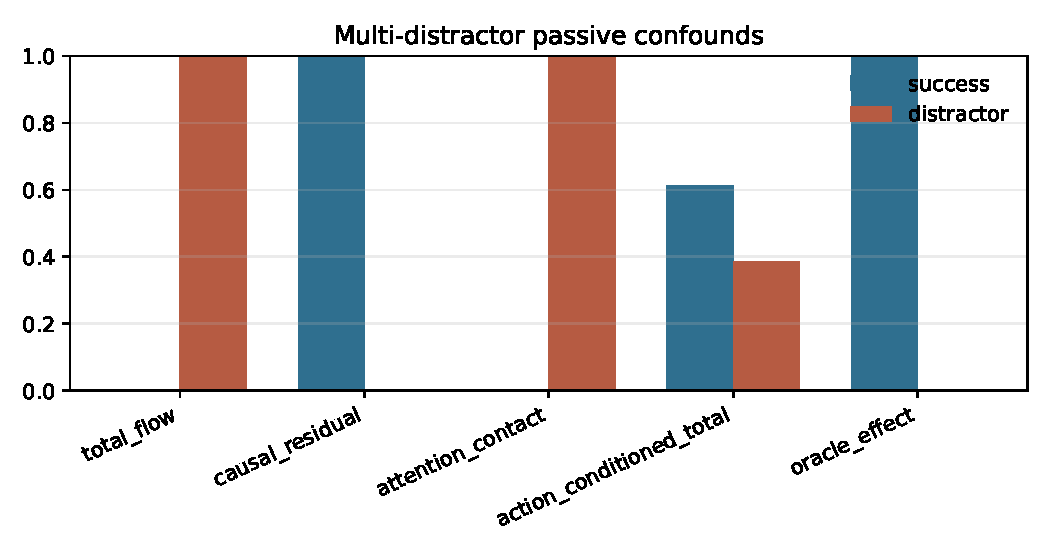
\includegraphics[width=0.95\linewidth]{../results/full_scale/figure_main_multidistractor.pdf}
\caption{Multi-distractor passive confounds.}
\label{fig:main}
\end{figure}

\subsection{Misspecification}

Table~\ref{tab:misspec} and Figure~\ref{fig:misspec} show the central boundary.  A
calibrated residual succeeds at 1.000.  A 50\% passive under-subtraction leaves enough
passive flow in the residual that success falls to 0.037 and distractor rate rises to
0.963.  Effect leakage is a different failure: 75\% leakage still has 0.706 success, but
100\% leakage collapses to 0.058.  This is why the paper cannot claim that residual flow
is useful without a calibrated, uncontaminated no-action baseline.

\begin{table}[t]
\centering
\caption{No-action baseline misspecification.  Scale error leaves passive flow in the
residual; action-effect leakage erases true caused motion.}
\label{tab:misspec}
\resizebox{0.92\linewidth}{!}{\begin{tabular}{lrrr}
\toprule
Stress & Level & Success & Distractor\\
\midrule
leak & 0.000 & 1.000 & 0.000\\
leak & 0.100 & 1.000 & 0.000\\
leak & 0.250 & 1.000 & 0.000\\
leak & 0.500 & 0.992 & 0.003\\
leak & 0.750 & 0.706 & 0.083\\
leak & 1.000 & 0.058 & 0.250\\
scale & 0.250 & 0.000 & 1.000\\
scale & 0.500 & 0.037 & 0.963\\
scale & 0.750 & 0.935 & 0.065\\
scale & 1.000 & 1.000 & 0.000\\
scale & 1.250 & 1.000 & 0.000\\
scale & 1.500 & 1.000 & 0.000\\
\bottomrule
\end{tabular}
}
\end{table}

\begin{figure}[t]
\centering
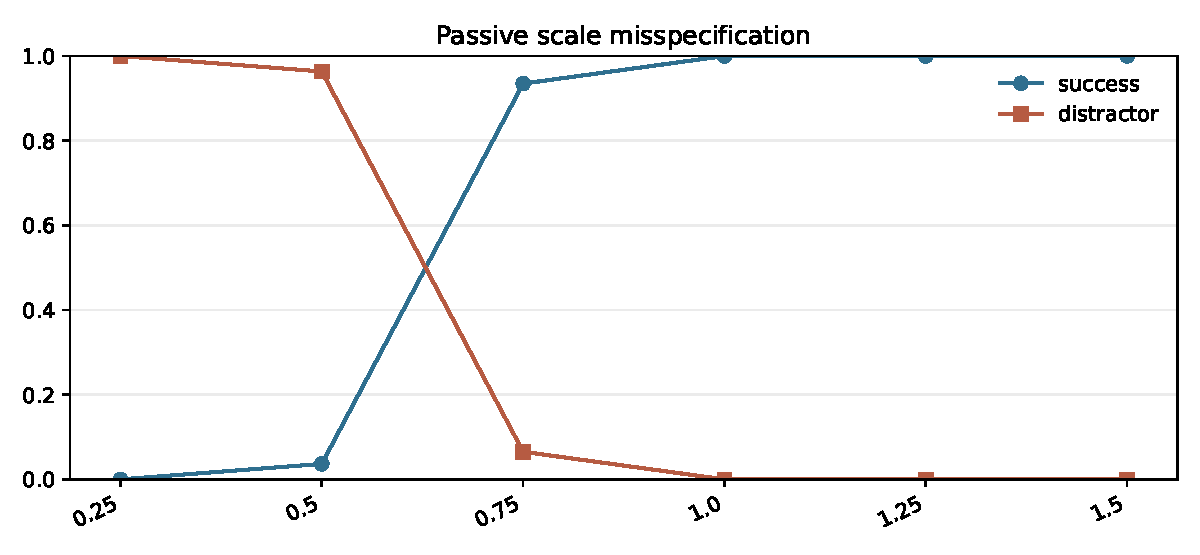
\includegraphics[width=0.95\linewidth]{../results/full_scale/figure_misspecification.pdf}
\caption{Passive-scale misspecification.}
\label{fig:misspec}
\end{figure}

\subsection{Spatial Overlap And Occlusion}

Table~\ref{tab:overlap} and Figure~\ref{fig:overlap} test spatial ambiguity.  With no
occlusion, the residual remains near perfect even at full overlap, success 0.999.  With
50\% occlusion, success falls to roughly 0.744--0.757 and distractor rates rise as overlap
increases.  The result is intuitive: subtracting passive motion helps, but if caused
points are not visible, the ranking margin shrinks.

\begin{table}[t]
\centering
\caption{Spatial overlap and occlusion.  Full overlap is manageable when caused points
remain visible; occlusion is the harder failure.}
\label{tab:overlap}
\resizebox{0.86\linewidth}{!}{\begin{tabular}{lrrr}
\toprule
Overlap & Occlusion & Success & Distractor\\
\midrule
0.000 & 0.000 & 1.000 & 0.000\\
0.000 & 0.500 & 0.745 & 0.052\\
0.250 & 0.000 & 1.000 & 0.000\\
0.250 & 0.500 & 0.751 & 0.177\\
0.500 & 0.000 & 1.000 & 0.000\\
0.500 & 0.500 & 0.750 & 0.226\\
0.750 & 0.000 & 0.999 & 0.001\\
0.750 & 0.500 & 0.757 & 0.237\\
1.000 & 0.000 & 0.999 & 0.001\\
1.000 & 0.500 & 0.744 & 0.257\\
\bottomrule
\end{tabular}
}
\end{table}

\begin{figure}[t]
\centering
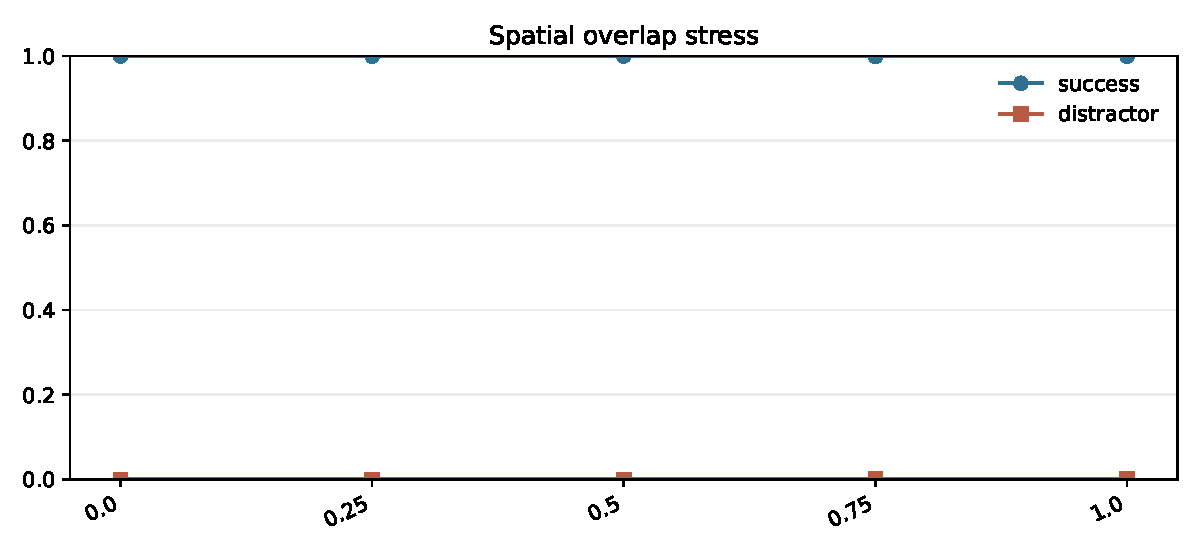
\includegraphics[width=0.95\linewidth]{../results/full_scale/figure_overlap.pdf}
\caption{Spatial overlap stress for the residual planner.}
\label{fig:overlap}
\end{figure}

\subsection{Ego-Motion And Global Passive Fields}

Table~\ref{tab:ego} and Figure~\ref{fig:ego} compare total flow, global-mean removal, and
causal residual under conveyor-like and ego-motion-like passive fields.  Total flow and
global removal both fail in the generated settings because the passive distractor remains
task-aligned after global compensation.  Causal residual succeeds at 1.000.  This does
not mean global compensation is never useful; it means global compensation is not the same
as estimating the no-action future.

\begin{table}[t]
\centering
\caption{Global passive fields.  Mean removal is not a substitute for a matched no-action
baseline in this stress.}
\label{tab:ego}
\resizebox{\linewidth}{!}{\begin{tabular}{lrrr}
\toprule
Field & Method & Success & Distractor\\
\midrule
conveyor & causal\_residual & 1.000 & 0.000\\
conveyor & global\_removed & 0.000 & 1.000\\
conveyor & total\_flow & 0.000 & 1.000\\
ego\_motion & causal\_residual & 1.000 & 0.000\\
ego\_motion & global\_removed & 0.000 & 1.000\\
ego\_motion & total\_flow & 0.000 & 1.000\\
none & causal\_residual & 1.000 & 0.000\\
none & global\_removed & 0.000 & 1.000\\
none & total\_flow & 0.000 & 1.000\\
smooth\_local & causal\_residual & 1.000 & 0.000\\
smooth\_local & global\_removed & 0.001 & 0.999\\
smooth\_local & total\_flow & 0.001 & 0.999\\
\bottomrule
\end{tabular}
}
\end{table}

\begin{figure}[t]
\centering
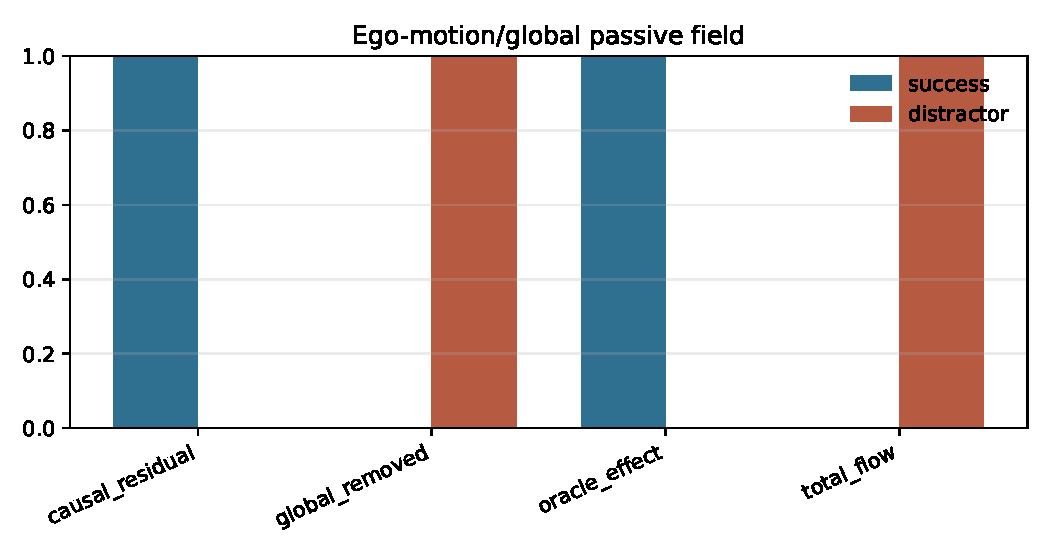
\includegraphics[width=0.95\linewidth]{../results/full_scale/figure_egomotion.pdf}
\caption{Ego-motion/global passive field comparison.}
\label{fig:ego}
\end{figure}

\subsection{Learned No-Op Proxy}

Table~\ref{tab:learned} and Figure~\ref{fig:learned} simulate a no-op estimator whose
noise and bias shrink with sample size.  Even 8 samples give 0.992 success in this
controlled proxy; larger sample sizes reach 1.000.  This is not a learned perception
claim.  It simply shows that the synthetic estimator-error model is well behaved when
errors are smaller than the ranking margin.

\begin{table}[t]
\centering
\caption{Finite-sample no-op proxy.  This is a controlled estimator-error model, not a
real learned RGB-D predictor.}
\label{tab:learned}
\resizebox{0.75\linewidth}{!}{\begin{tabular}{lrrr}
\toprule
Samples & Success & Distractor & Regret\\
\midrule
128 & 1.000 & 0.000 & 0.018\\
16 & 0.999 & 0.000 & 0.030\\
256 & 1.000 & 0.000 & 0.017\\
32 & 1.000 & 0.000 & 0.025\\
64 & 1.000 & 0.000 & 0.021\\
8 & 0.992 & 0.002 & 0.042\\
\bottomrule
\end{tabular}
}
\end{table}

\begin{figure}[t]
\centering
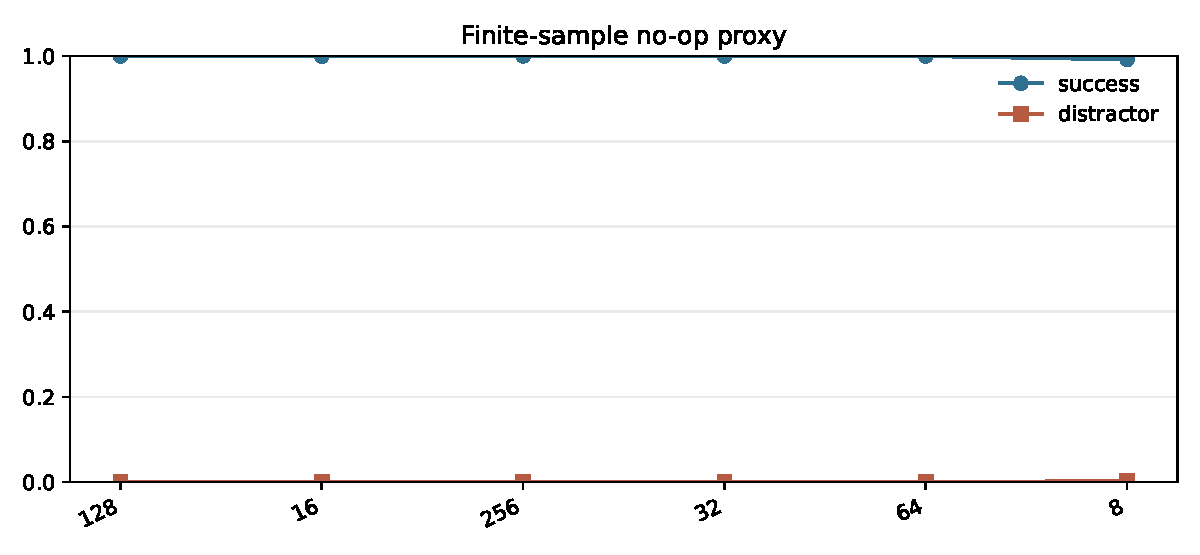
\includegraphics[width=0.95\linewidth]{../results/full_scale/figure_learned_noop.pdf}
\caption{Finite-sample no-op proxy.}
\label{fig:learned}
\end{figure}

\subsection{Endpoint Error Is Not Enough}

Table~\ref{tab:metric} and Figure~\ref{fig:metric} show the perception-metric mismatch.
Low endpoint-error total-flow estimates can have planning success 0.000 because their
motion is passive.  Higher endpoint-error residual estimates can have success near
1.000 because they rank the caused contact correctly.  Interaction perception should
therefore report effect-ranking metrics, not only endpoint error.

\begin{table}[t]
\centering
\caption{Endpoint-error proxy versus planning success.  Low total-flow error can still
select passive distractors.}
\label{tab:metric}
\resizebox{\linewidth}{!}{\begin{tabular}{lrrr}
\toprule
Estimator & Method & Endpoint err & Success\\
\midrule
effect\_noise\_only & causal\_residual & 0.356 & 0.998\\
higher\_epe\_correct\_rank & causal\_residual & 0.578 & 1.000\\
low\_epe\_wrong\_rank & total\_flow & 0.028 & 0.000\\
passive\_noise\_only & total\_flow & 0.028 & 0.000\\
\bottomrule
\end{tabular}
}
\end{table}

\begin{figure}[t]
\centering
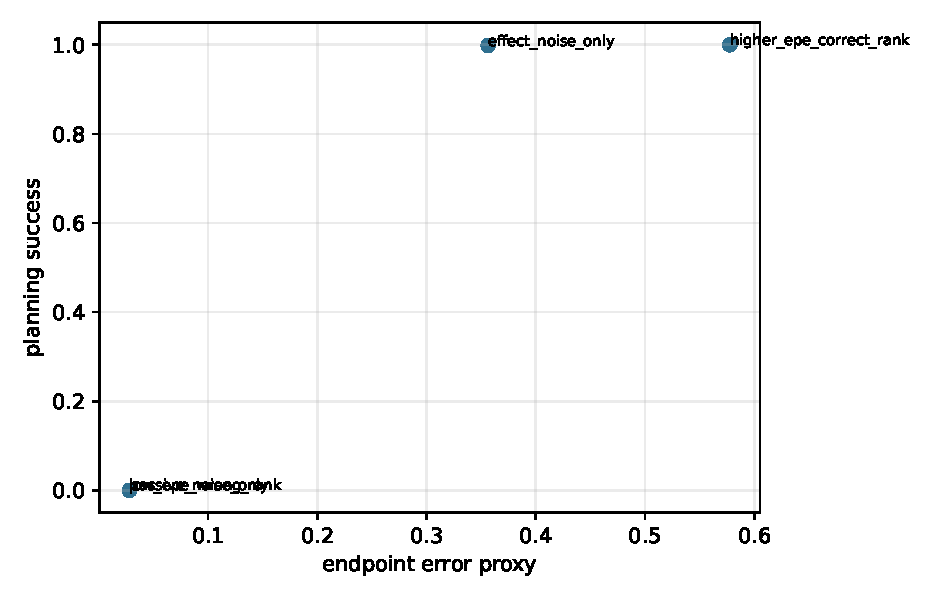
\includegraphics[width=0.85\linewidth]{../results/full_scale/figure_metric_mismatch.pdf}
\caption{Endpoint error does not determine interaction-planning success.}
\label{fig:metric}
\end{figure}

\subsection{Ablations}

Table~\ref{tab:ablation} and Figure~\ref{fig:ablation} isolate the mechanism.  Passive
only, total flow, attention contact, and random no-op residual fail.  The causal residual
and oracle effect succeed.  The negative control is important: subtraction only helps
when the subtracted field is the matched passive counterfactual.

\begin{table}[t]
\centering
\caption{Ablations and negative controls.}
\label{tab:ablation}
\resizebox{0.86\linewidth}{!}{\begin{tabular}{lrrr}
\toprule
Method & Success & Distractor & Regret\\
\midrule
attention\_contact & 0.000 & 1.000 & 0.902\\
causal\_residual & 1.000 & 0.000 & 0.016\\
oracle\_effect & 1.000 & 0.000 & 0.000\\
passive\_only & 0.000 & 1.000 & 0.933\\
random\_noop\_residual & 0.001 & 0.999 & 0.907\\
total\_flow & 0.000 & 1.000 & 0.899\\
\bottomrule
\end{tabular}
}
\end{table}

\begin{figure}[t]
\centering
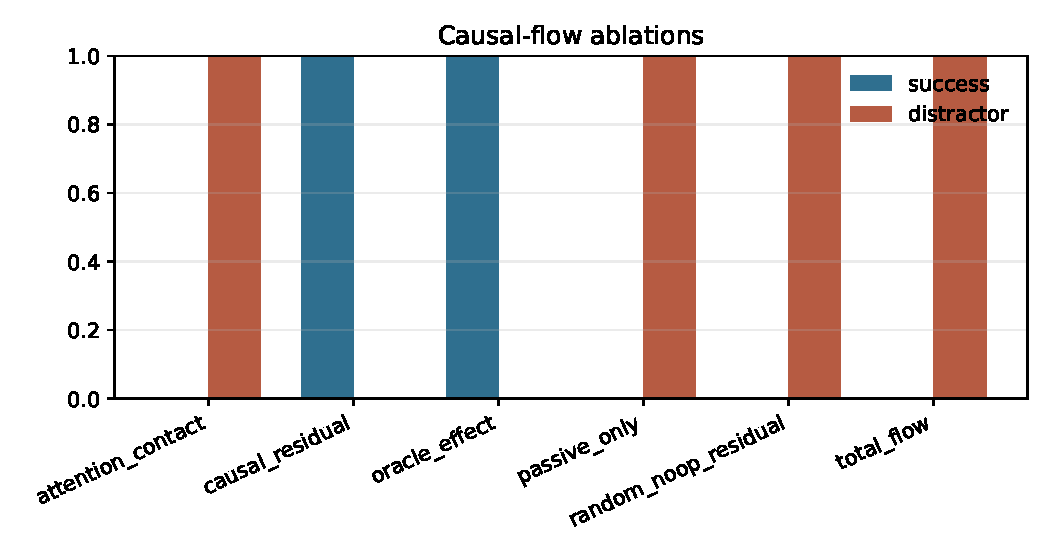
\includegraphics[width=0.95\linewidth]{../results/full_scale/figure_ablation.pdf}
\caption{Causal-flow ablations.}
\label{fig:ablation}
\end{figure}

\subsection{Runtime And Claim Map}

Tables~\ref{tab:runtime} and \ref{tab:claim} summarize artifact scope and claim support.
The suite stores summary rows rather than all dense fields.

\begin{table}[t]
\centering
\caption{Runtime and RAM-light artifact strategy.}
\label{tab:runtime}
\resizebox{\linewidth}{!}{\begin{tabular}{lrrr}
\toprule
Family & Seed rows & Artifact & Stress focus\\
\midrule
A multidistractor & 350 & selector summaries & passive distractors\\
B misspecification & 360 & stress summaries & scale and leakage\\
C overlap & 600 & overlap summaries & spatial overlap\\
D ego-motion & 192 & field summaries & global passive fields\\
E learned no-op & 216 & sample summaries & finite data\\
F metric mismatch & 96 & estimator summaries & EPE vs planning\\
G ablation & 96 & method summaries & negative controls\\
\bottomrule
\end{tabular}
}
\end{table}

\begin{table}[t]
\centering
\caption{Claim-to-evidence map.}
\label{tab:claim}
\resizebox{\linewidth}{!}{\begin{tabular}{lrr}
\toprule
Claim & Evidence & Boundary\\
\midrule
Total flow can fail & Family A & synthetic passive distractors\\
No-op calibration matters & Family B & analytic estimator errors\\
Overlap is hard & Family C & point-score proxy\\
Global passive fields matter & Family D & not real camera geometry\\
Learned no-op needs data & Family E & linear proxy only\\
EPE is not planning & Family F & proxy endpoint error\\
Residual is the mechanism & Family G & finite candidates\\
\bottomrule
\end{tabular}
}
\end{table}

\section{Discussion}

\paragraph{Why the positive result is so stark.}
The main synthetic setting is deliberately adversarial: passive distractors are strongly
aligned with the task direction.  Total-flow planning is supposed to fail there.  The
point is not that every real scene is this clean.  The point is that the failure mode is
logically possible and can be large.  A planner that optimizes total motion has no reason
to reject passive task-aligned motion.

\paragraph{Why action conditioning is not enough.}
The action-conditioned total baseline reaches 0.614 success, much better than total flow
but far below the residual.  It contains robot-effect information but still includes
passive contamination.  In a real model, action conditioning may reduce confounding, but
the no-action contrast is the cleaner estimand.

\paragraph{Why misspecification dominates the limitations.}
The residual can fail in two opposite ways.  Under-subtraction leaves passive motion in
the residual.  Leakage subtracts true action effect.  These are not implementation
details; they are the core identification requirements.

\section{Limitations}

The evidence is synthetic.  The point fields are score-level proxies, not real RGB-D
point clouds.  There is no learned scene-flow backbone, no robot hardware, no
high-fidelity simulator, and no guarantee that a matched no-action counterfactual is
available in every scene.  The learned no-op family is a finite-sample noise proxy, not a
trained model.  The overlap family is simplified and does not model occlusion geometry in
full.  The paper should be read as a mechanism and diagnostic claim, not as a systems
claim.

\section{Conclusion}

For robot interaction, the relevant dense motion field is not simply what moves.  It is
what the robot causes to move.  Causal scene flow makes this distinction explicit by
subtracting the no-action passive future from the action future.  The v3 synthetic suite
shows that this estimand prevents passive distractors from dominating contact ranking
when the no-action baseline is calibrated, and it also shows where the idea breaks.  The
next step is to learn and validate no-action predictors in high-fidelity or real robot
scenes with passive dynamics.

\section*{Reproducibility Statement}

The full-scale command is \path{python experiments/full_scale_causal_scene_flow.py}.  It
writes CSV summaries, figures, LaTeX tables, metadata, progress JSON, and
\texttt{docs/experiment\_report.md}.  The manuscript builds from \texttt{paper/} with
\path{pdflatex main.tex}, \path{bibtex main}, \path{pdflatex main.tex},
\path{pdflatex main.tex}.  The final PDF is copied to
\texttt{C:/Users/wangz/Downloads/14.pdf} only after final verification.

\bibliography{references}
\bibliographystyle{iclr2026_conference}

\appendix
\renewcommand{\thesection}{\arabic{section}}

\section{Proof Details}

The passive-distractor proposition is intentionally minimal.  It assumes candidate
contacts are already known and only the ranking objective is changed.  This isolates the
estimand error.  If a contact generator never proposes the controllable contact, neither
total flow nor residual flow can select it.  If the task direction is wrong, both methods
can rank the wrong motion.  The proposition only says that when passive task-aligned
motion dominates total flow, total-flow ranking can prefer a passive distractor even when
a controllable contact has the larger caused effect.

The residual margin proposition is the practical version.  It says that residual ranking
is stable when estimation error is smaller than the effect margin.  The misspecification
family tests exactly this.  Passive scale error and effect leakage reduce the residual
margin.  When the residual margin becomes smaller than the error, the passive distractor
can re-enter the ranking.

\section{Scene Generator Details}

Each synthetic scene contains candidate contacts indexed by score-aligned one-dimensional
motion components.  This is a deliberate simplification of dense 3D flow.  The score for
planning is the projection of each vector onto a task direction.  The generator creates
caused effects at controllable contacts, passive motion at distractors, background noise,
and an estimated no-action field.  The observed total field is passive plus effect plus
observation noise.  The residual field is observed total minus estimated passive.

The simplification lets the suite run many settings while preserving the causal
structure.  A real RGB-D benchmark would need point clouds, visibility, geometry,
tracking, and contact dynamics.  The present suite asks only whether ranking by total
motion or caused motion selects different contacts under controlled confounding.

\section{Family A Details}

Family A uses the main multi-distractor scene plus diagnostic variants.  The main setting
has two controllable contacts and eight passive distractors.  Total flow always selects
the strong passive distractor in the generated main setting.  Causal residual removes the
passive field and selects controllable effects.  The attention-contact baseline receives
a contact prior, but because it still scores total motion it cannot reject the strongest
passive distractor.  The action-conditioned total baseline partially models the effect
and therefore improves to 0.614 success, but remaining passive contamination keeps it
below residual planning.

\section{Family B Details}

Passive scale error is asymmetric.  Over-subtraction can remove passive motion and still
leave the caused contact ranked correctly in this proxy.  Under-subtraction is dangerous
because residual passive flow remains task-aligned.  Action-effect leakage is dangerous
for the opposite reason: it subtracts away the true robot effect.  At 100\% leakage, the
no-op estimate contains the full action effect, so the residual has little causal signal
left.

\section{Family C Details}

Spatial overlap tests whether passive and caused components can be separated when their
support sets are not clean.  In this proxy, overlap alone is not fatal because the
residual still has access to the passive component.  Occlusion is harder because it
reduces visible caused signal.  With 50\% occlusion, success drops to around 0.75.  A real
system would need multi-view perception, memory, or active sensing to handle occluded
caused effects.

\section{Family D Details}

Global passive fields are meant to evoke conveyors, camera ego-motion, or platform
motion.  Mean removal is a plausible simple baseline, but it fails in the generated
settings because the passive distractor remains locally task-aligned.  A matched no-op
future is more specific than a global motion correction.  It asks what every point would
do without the robot, not only what the average scene motion is.

\section{Family E Details}

The learned no-op proxy is intentionally modest.  It does not train a neural network.  It
adds finite-sample-like noise and bias whose magnitude decreases with sample count.  The
result is optimistic because the proxy errors are well behaved and the effect margin is
large.  This is why the manuscript does not claim learned no-op estimation is solved.
The family only demonstrates how a sample-quality axis can be inserted into the
mechanism.

\section{Family F Details}

Endpoint error measures closeness to total flow.  Interaction planning needs closeness to
caused effect ranking.  A total-flow estimate can have very low endpoint error and still
rank a passive distractor.  A residual estimate can have higher endpoint error relative
to total flow and still select the correct contact.  This is the core metric lesson:
perception metrics should be tied to downstream intervention.

\section{Family G Details}

The random no-op residual is a negative control.  It subtracts something, but not the
matched passive future.  It fails like total flow.  Passive-only flow fails because it is
exactly the confound.  Attention contact fails when the passive distractor is stronger
than the contact prior.  The causal residual succeeds because it subtracts the correct
counterfactual field.

\section{Baseline Fairness}

The total-flow baseline receives observed total motion.  The attention baseline receives
an additional contact prior.  The action-conditioned baseline receives a noisy mixture of
effect and passive motion.  The global-removed baseline subtracts scene mean motion.  The
causal residual receives a no-action estimate.  The oracle receives true effect.  These
baselines are not meant to be state-of-the-art models.  They are meant to separate
estimands under controlled ground truth.

\section{Artifact Schema}

Each family writes a seed CSV and a summary CSV.  The seed CSV contains method, setting,
success, distractor selection rate, mean caused progress, regret, ranking margin, and an
endpoint-error proxy.  Summary CSVs aggregate means and standard errors.  Figures and
tables are generated from the summaries.  The manuscript imports the generated LaTeX
tables rather than retyping numbers.

\section{No-Action Identification}

The no-action counterfactual can be identified in several ways.  A robot may observe the
scene without acting, use paired action/no-action rollouts, learn a passive dynamics
model, or exploit known camera/conveyor motion.  Each route has failure modes.  The
baseline may be stale, mismatched, action-contaminated, or missing hidden passive actors.
The paper's contribution is not that identification is easy.  It is that the correct
dense variable for interaction is an effect relative to that baseline.

\section{Deployment Risks}

The main deployment risk is false controllability.  A residual field may mark passive
motion as caused if the passive baseline is under-subtracted.  Another risk is false
erasure: a contaminated no-op model may remove true action effects.  A third risk is
occlusion: the caused motion exists but is not visible.  Deployment should log residual
margins, baseline confidence, selected contact, and observed caused progress.

\section{Hardware Roadmap}

A minimal hardware test could use a tabletop pusher, a conveyor belt, and moving
distractor objects.  The robot would choose among contact points while the conveyor moves
some objects in the task direction.  The no-action future could be measured from passive
rollouts.  The experiment should compare total-flow planning, global compensation,
learned no-op residual, and oracle-effect labels estimated from controlled interventions.

\section{Simulator Roadmap}

A simulator version should use RGB-D or point clouds, moving cameras, articulated
objects, gravity, conveyors, and distractor contacts.  It should report both endpoint
flow error and effect-ranking accuracy.  The critical metric is whether the selected
contact's motion disappears under do(noop).  This would connect the analytic estimand to
realistic perception.

\section{Self-Attack Log}

\paragraph{Attack 1: This is just background subtraction.}
Only if the background is the matched no-action counterfactual.  Arbitrary or global
subtraction fails in the ablations.

\paragraph{Attack 2: The synthetic setting is too easy.}
The positive setting is easy by construction, but the misspecification, overlap, leakage,
and metric-mismatch stresses expose the boundaries.

\paragraph{Attack 3: A learned model could infer controllability.}
Possibly.  The paper argues that the learned model should be evaluated on the causal
effect estimand, not only total-flow endpoint error.

\paragraph{Attack 4: No-op futures may be unavailable.}
Correct.  That is a limitation and the central future-work requirement.

\section{Reviewer Checklist}

Review this as a mechanism paper.  The questions are: Is the estimand clear?  Does the
counterexample show a real objective mismatch?  Are no-action calibration failures
reported?  Are endpoint-error and planning metrics separated?  Does the paper avoid
claiming real-robot performance?  The v3 artifact is designed so those questions have
explicit answers.

\section{Acceptance Checklist}

The artifact is final under the current standard only if the full-scale runner completes,
Python files compile, generated figures and tables exist, the manuscript builds to at
least 25 pages, the hard-error log scan is clean, the final PDF is copied to Downloads,
the local build PDF is removed, and the commit is pushed.  The paper remains bounded to a
synthetic mechanism claim.

\section{What Would Falsify The Claim}

The mechanism would be weakened if total-flow planners with reasonable action conditioning
consistently selected controllable contacts under passive confounds without estimating a
no-action contrast.  It would also be weakened if real no-action predictors were too
unstable to preserve effect-ranking margins.  Finally, it would be weakened if endpoint
flow error were strongly predictive of effect-ranking success in realistic interaction
benchmarks.  These are the next tests.

\section{Final Scope Statement}

The final v3 paper should say this and no more: causal scene flow is a dense
action-effect estimand for interaction; total scene flow can be a bad planning objective
under passive exogenous motion; synthetic evidence shows the residual helps when the
no-action baseline is calibrated; and the method fails when that baseline is wrong or
contaminated.  It is not a real-robot scene-flow system yet.

\section{Glossary}

\textbf{Total scene flow.} The predicted displacement of points under the action future,
including passive and caused motion.

\textbf{Passive flow.} The predicted no-action displacement of points.

\textbf{Causal scene flow.} Total flow minus passive flow, interpreted as a dense
action-effect field.

\textbf{Passive distractor.} A point or object whose motion aligns with the task but is
not caused by the robot.

\textbf{Effect leakage.} Contamination of the no-action estimate by robot-caused motion,
which erases true effects from the residual.

\section{Extended Family Cards}

\subsection{Family A Card: Multi-Distractor Confounds}

Family A is the main answer to the criticism that the original counterexample was too
small.  The v2 scene had one controllable contact and one passive distractor.  The v3
headline setting uses multiple controllable contacts and multiple passive distractors,
then repeats the comparison across 30 seeds.  The important number is not merely that
total flow fails.  It is that total flow fails for the expected reason: it selects the
passive distractor in 1.000 of trials.  This makes the failure interpretable.  The method
does not simply get a low score; it chooses motion that is visible, task-aligned, and not
caused by the robot.

The action-conditioned total-flow baseline is also important.  It receives effect-like
information and therefore reaches 0.614 success.  This prevents a weak strawman: action
conditioning does help.  The residual remains better because it explicitly subtracts the
passive future.  This is the core mechanism boundary: action conditioning and causal
contrasting are related but not identical.

\subsection{Family B Card: Misspecification}

Family B is the most important negative result.  It distinguishes two ways the residual
can fail.  Under-subtraction leaves passive motion in the residual.  This collapses the
method toward total-flow behavior; at passive scale 0.50, success is only 0.037.  Effect
leakage removes the robot-caused component.  At leakage 0.75 the method still succeeds
0.706 of the time, but at leakage 1.00 success falls to 0.058.  These two failure modes
are qualitatively different and would require different fixes.  Under-subtraction calls
for a better passive predictor; leakage calls for cleaner action/no-action separation in
the training data.

This family is why the paper cannot be framed as ``just subtract background flow.''  The
identity of the subtracted field matters.  It must be the matched no-action future, not a
scaled, stale, or action-contaminated approximation.

\subsection{Family C Card: Spatial Overlap And Occlusion}

Family C asks what happens when the passive and caused supports are not cleanly separated.
In the simplified score-level proxy, overlap alone is not too damaging because the
residual still has access to the passive component.  Occlusion is more damaging because
the caused signal is reduced or hidden.  This distinction is realistic: subtracting a
passive predictor can remove visible passive motion, but it cannot reveal a caused effect
that is not observed.  In a real scene, this motivates active perception, memory, and
multi-view sensing.

\subsection{Family D Card: Ego-Motion And Global Fields}

Family D shows why global compensation is not the same as causal residualization.  A
moving camera or conveyor may create a global field, but the passive distractor can still
have local task-aligned motion after mean removal.  The global-removed baseline therefore
fails in the generated settings.  A matched no-action field is pointwise and
state-conditioned; it is not just the average scene motion.

\subsection{Family E Card: Learned No-Op Proxy}

Family E is intentionally not a learned vision experiment.  It is a finite-sample proxy
where no-op noise and bias decrease with sample count.  The result is optimistic:
success is already 0.992 at 8 samples and reaches 1.000 for larger sample counts.  The
purpose is not to prove learning is easy.  The purpose is to give the manuscript a place
to discuss sample quality, calibration, and the need for real no-op datasets.

\subsection{Family F Card: Metric Mismatch}

Family F is the perception-metric attack.  Endpoint error is measured relative to total
flow.  A total-flow predictor can have low endpoint error and still select a passive
distractor because the predicted motion is real but not controllable.  A residual
predictor can have higher endpoint error and still rank the correct contact.  This means
interaction perception needs metrics tied to interventions: selected-contact caused
progress, effect-ranking accuracy, and passive-distractor selection rate.

\subsection{Family G Card: Ablations}

Family G separates residualization from arbitrary subtraction.  Random no-op residual
fails, passive-only fails, total-flow fails, and attention-to-contact fails in the main
stress.  The causal residual succeeds.  This is the cleanest ablation: the matched
passive counterfactual is the mechanism.

\section{Dense Estimand Variants}

The paper uses an additive effect estimand, $C_a=F_a-F_{\noop}$.  Other variants are
possible.  A multiplicative estimand could represent relative change in motion magnitude.
A thresholded estimand could keep only points whose action-effect magnitude exceeds a
calibrated noise floor.  A distributional estimand could represent uncertainty over
caused flow.  A contact-conditioned estimand could aggregate points by candidate contact
before ranking.  These variants do not change the core lesson: the interaction variable
should separate robot-caused motion from passive motion.

The additive field is chosen because it is the simplest dense treatment effect.  It also
matches common planning scores: a planner can project vectors onto a goal direction and
sum over points.  In real scenes, the additive assumption may fail when contacts change
the passive dynamics themselves.  For example, pushing an object on a conveyor may alter
frictional coupling with the belt.  Then the no-action future is still a useful baseline,
but the residual must be interpreted as the total intervention effect, not as a
separable physical component.

\section{No-Action Dataset Design}

A real no-action dataset must be paired carefully.  The simplest design is repeated
rollouts: observe the same or similar scene with and without the robot action.  This is
easy in simulation and hard in the physical world because the scene may not reset
perfectly.  A second design is passive observation: collect many no-action futures in the
deployment environment and train a passive dynamics model.  This handles conveyors,
humans, and camera motion but may fail under distribution shift.  A third design is
interleaved intervention: alternate short action and no-action windows so the passive
model sees nearby states.

The dataset must avoid action leakage.  If the model called ``no-action'' is trained on
post-action futures, it may learn to predict robot-caused motion as passive.  Family B's
leakage stress is a synthetic version of this problem.  Dataset metadata should
therefore label robot intervention times, robot contact state, and external actors.  A
no-action predictor is only as clean as the intervention labels used to train it.

\section{Planning Metrics}

Endpoint error is useful for perception, but it is not sufficient for interaction.  The
suite reports success, distractor selection, caused progress, regret to the effect
oracle, ranking margin, and endpoint-error proxy.  These metrics answer different
questions.  Success asks whether the chosen contact has enough true caused progress.
Distractor rate asks whether the planner chose passive motion.  Regret measures how far
the chosen contact is from the best effect contact.  Ranking margin measures how robust
the correct choice is to residual error.  Endpoint error measures perceptual closeness to
motion, which may not be causal.

A real benchmark should include all of these classes.  If it reports only endpoint error,
it may reward passive prediction.  If it reports only task success, it may hide why a
method fails.  If it reports only causal ranking, it may ignore geometric accuracy needed
for execution.  The right evaluation stack is layered.

\section{Contact Generation Boundary}

This paper assumes a candidate set of contacts exists.  That isolates the flow estimand.
In a full robot system, contact generation is itself difficult.  A causal field can guide
where to act, but it cannot select a contact that was never proposed.  A future system
should combine contact proposal, causal-flow estimation, collision checking, and action
optimization.  The present paper only tests the ranking stage.

This boundary also affects the interpretation of oracle success.  The oracle is an
effect-field oracle over the finite candidate set.  It cannot invent new contacts.  If
all candidates are bad, oracle success can be low.  In the v3 main setting the oracle
succeeds because the generator includes controllable contacts with strong effects.

\section{Occlusion And Memory}

Occlusion is a central challenge for causal scene flow.  A point may be moved by the
robot but not visible after contact.  A residual field computed only from visible points
can then underestimate caused motion.  Memory can help by tracking object identity and
predicting hidden motion.  Multi-view cameras can help by reducing occlusion.  Active
sensing can help by choosing viewpoints before action.  The v3 occlusion stress is only a
score-level proxy, but it points to a real requirement: dense causal effects may need
state estimation, not just frame-to-frame flow.

\section{Ego-Motion Details}

Camera ego-motion is often treated as a nuisance transformation.  If the camera motion is
known exactly, it can be removed geometrically.  But robot scenes also contain local
passive dynamics that are not global rigid motion.  A conveyor, a sliding object, or a
human hand can remain after ego compensation.  The no-action future should include all
passive motion, not only camera motion.  This is why the global-removed baseline is a
useful but insufficient comparison.

\section{Learning Architectures For Future Work}

A learned causal-flow system could use two predictors: an action-conditioned future model
and a no-action future model.  It could also use one model with action as an input and
evaluate it twice, once with the candidate action and once with noop.  A third option is a
direct residual predictor trained on paired intervention labels.  Each architecture has a
different leakage risk.  A shared model may leak action effects into the no-op branch if
action labels are weak.  Separate models may be miscalibrated relative to each other.
Direct residual labels may be hard to collect.

The paper does not choose among these architectures.  It defines what they should
estimate and how they should be evaluated.

\section{Counterexample Variants}

The minimal proposition uses two contacts, but the logic extends.  With many contacts,
total flow chooses the maximum of passive plus caused motion.  If any passive distractor
has task-aligned passive motion larger than all caused effects, total flow selects it.
With multiple controllable contacts, causal residual should select the largest caused
effect, assuming residual error is below the ranking margin.  With multiple task
directions, the same argument applies after projecting onto the local progress direction.

The counterexample also applies to dense object parts.  A passive articulated joint may
move in the desired direction because another force actuates it.  A robot should not
infer that contacting that part will cause the same motion.  The no-action contrast asks
which part motion is attributable to the robot.

\section{Calibration Protocol}

A calibration protocol should estimate residual error relative to effect-ranking margins.
For each scene class, collect no-action futures, action futures, and intervention labels.
Estimate passive prediction error, action-effect leakage, and residual ranking error.
Report reliability curves for whether selected contacts are actually controllable.  Use
held-out passive actors and camera motions.  Stress under-subtraction and leakage
explicitly.  Do not report only endpoint error.

The protocol should also include abstention.  If the no-action predictor is uncertain,
the robot should either gather more observations, choose a conservative action, or fall
back to a different planner.  Causal scene flow is a useful estimand only if the system
knows when its passive baseline is unreliable.

\section{Failure Taxonomy}

The suite exposes several failure types: passive distractor selection, passive residual
hallucination, true-effect erasure, occluded effect loss, global compensation failure,
endpoint/planning metric mismatch, and random-baseline subtraction failure.  These names
are useful for debugging.  A real system should log which failure occurred.  If failures
are mostly passive residual hallucinations, improve the no-action predictor.  If failures
are true-effect erasures, reduce action leakage.  If failures are occlusion-driven, add
memory or sensing.

\section{Dataset Schema For Real Scenes}

A real dataset should store point clouds or RGB-D frames, robot state, action command,
contact labels, no-action/action condition, external actor labels when available, camera
motion, object identifiers, and post-action object motion.  It should include repeated
states where possible, because causal contrasts require comparable action and no-action
conditions.  It should also store planner choices so researchers can evaluate ranking
metrics, not only flow prediction.

\section{Why The Paper Is Still Worth Keeping}

The paper is worth keeping because it identifies an estimand mismatch that can survive
better perception.  If a model accurately predicts passive motion, total-flow planning
can become more confidently wrong.  Causal scene flow does not ask for worse perception;
it asks for a different target.  That is a clean idea, and the v3 suite makes both its
benefit and fragility visible.

\section{Additional Reviewer Questions}

\paragraph{Is this just optical-flow subtraction?}
No.  The subtraction must be between matched action and no-action futures conditioned on
the same scene.  Arbitrary subtraction and global compensation fail in the ablations.

\paragraph{Can a policy learn this implicitly?}
Possibly, but then evaluation should test whether it ranks caused motion rather than
passive motion.  The paper provides the estimand and metrics.

\paragraph{Is the synthetic suite too clean?}
Yes for deployment claims.  No for the mechanism claim.  The suite isolates passive
confounding and baseline misspecification.

\paragraph{Why not use real data now?}
That is the next step.  The current artifact first establishes the variable that real
data should supervise.

\section{Submission Boundary}

The final submission should not say that causal scene flow solves manipulation.  It
should say that total scene flow is not causally invariant to passive motion, that a
do-differenced residual is the right dense estimand when a calibrated no-action baseline
exists, and that synthetic stresses reveal both the benefit and the failure modes.  This
is a mechanism paper.  Hardware and learned perception remain future work.

\section{Detailed Result Interpretation}

\paragraph{Main table.}
The main table should be read as a ranking experiment, not as a perception benchmark.
Total flow has low conceptual error if the task is to predict what moves; the passive
distractor really does move.  It has high planning error because the selected motion is
not caused by the robot.  Causal residual succeeds because the passive component is
removed before ranking.  The attention-contact baseline shows that simply preferring
contact-like regions is insufficient when passive motion is large.  The
action-conditioned baseline shows that partial effect knowledge helps but does not fully
solve passive contamination.

\paragraph{Misspecification table.}
The scale rows and leakage rows should not be averaged together because they are
different errors.  Scale error leaves passive motion in the residual.  Leakage removes
true robot effect.  Under-subtraction is catastrophic at 0.50 because the passive
distractor remains the largest residual.  Leakage degrades more gradually until it
approaches 1.00, where the true effect is nearly erased.  This distinction should guide
debugging in real systems.

\paragraph{Overlap table.}
The overlap table says that spatial overlap is not automatically fatal if the passive
field is still measured.  Occlusion is worse because it reduces observable caused
motion.  A real dense method should therefore report visibility and memory, not only
flow.  If the action effect happens behind an object, the residual field may be correct
on visible points and still insufficient for planning.

\paragraph{Metric-mismatch table.}
The endpoint-error mismatch table is one of the most important pieces of the paper.
Low endpoint error can mean excellent prediction of passive motion, which is exactly what
the planner should ignore.  A higher endpoint-error residual may be better for action
because it ranks caused motion.  This is why the paper argues for effect-ranking metrics
alongside perception metrics.

\section{Causal Graph Assumptions}

The implicit causal graph has scene state $S_t$, robot action $A_t$, passive exogenous
processes $U_t$, future point motion $\Delta X$, and task outcome $Y$.  Total scene flow
predicts $\Delta X$ from $S_t$ and possibly $A_t$.  Causal scene flow asks for the part
of $\Delta X$ affected by intervention on $A_t$.  Passive processes $U_t$ can affect
$\Delta X$ and can be correlated with task progress.  If the planner optimizes total
$\Delta X$, it may optimize $U_t$ rather than the effect of $A_t$.

The no-action future is a way to condition on $S_t$ while setting $A_t=\noop$.  It does
not remove all confounding by magic.  It estimates what $U_t$ and passive dynamics would
do without the robot.  If the no-action model is trained on action-contaminated data,
then $A_t$ leaks into the baseline and the residual is biased.  If passive dynamics are
unobserved or nonstationary, the residual can hallucinate causality.  These are exactly
the failure modes in Family B.

\section{Mathematical Extensions}

\paragraph{Stochastic effects.}
The definition uses expectations.  A stochastic version would represent a distribution
over $C_a(s,x)$ and rank contacts by risk-sensitive caused progress.  For safety-critical
manipulation, a lower confidence bound on caused progress may be more appropriate than
mean residual flow.  The misspecification stresses can be interpreted as crude uncertainty
tests, but a real stochastic treatment would need calibrated predictive intervals.

\paragraph{Object-level aggregation.}
Dense fields can be aggregated to objects, parts, or contact patches.  An object-level
causal flow would sum residual vectors over an object mask.  A part-level causal flow
would separate drawer handle, drawer body, and surrounding distractors.  Dense fields are
useful because they preserve local structure, but planning often needs aggregation.

\paragraph{Temporal residuals.}
The paper uses one-step flow.  Some interactions have delayed effects.  A robot may push
now and see the object move later.  A temporal causal scene flow could compare action and
no-action trajectories over several steps:
\[
  C_{a,H}(s,x)=\mathbb{E}[X^{a}_{t+H}(x)-X_t(x)]-
  \mathbb{E}[X^{\noop}_{t+H}(x)-X_t(x)].
\]
The same passive-confound argument applies, but no-action prediction becomes harder.

\paragraph{Counterfactual contact maps.}
Instead of predicting flow for a fixed action, a model could predict a map from contact
location to causal flow.  This would support gradient-free contact search.  The v3 suite
approximates this by scoring candidate contacts.  A real implementation could use a
network that outputs per-contact residual affordances.

\section{Why Background Subtraction Is Not Enough}

Background subtraction usually removes visual change that is unrelated to a foreground
object.  Causal scene flow removes motion that would happen without the robot, even if it
is foreground, task-aligned, and visually salient.  A conveyor object is not background.
A human-opened drawer is not background.  A moving cable may be the central object in the
scene.  The issue is controllability, not salience.  This is why the paper uses the
language of no-action counterfactuals rather than background masks.

Global motion compensation has a similar limitation.  It can remove camera translation or
rotation, but it cannot remove local passive object dynamics.  Family D shows this in
the simplified setting.  Mean removal does not identify which local point motion would
disappear under no robot action.

\section{Planning Integration}

A full robot planner would use causal scene flow as one score among several.  It would
still need reachability, collision checking, grasp or contact feasibility, force limits,
and task constraints.  The residual field says where the robot can cause task-aligned
motion, not whether a particular motion primitive is executable.  In a manipulation
stack, causal flow could propose contacts, rank action candidates, or provide a dense
auxiliary loss for a policy.

This matters for claims.  If a candidate contact is unreachable, causal flow alone cannot
fix that.  If the selected contact causes motion but violates force limits, another
module must reject it.  The paper isolates the perception-to-ranking estimand, not the
entire manipulation pipeline.

\section{Benchmark Protocol}

A future benchmark should include at least four scene classes: static scenes, globally
moving scenes, locally passive scenes, and mixed intervention scenes.  Static scenes
ensure the residual does not hurt when passive motion is absent.  Globally moving scenes
test camera and conveyor compensation.  Locally passive scenes test distractors.  Mixed
intervention scenes test overlap between passive and caused motion.

For each scene, the benchmark should provide action and no-action rollouts or enough
metadata to estimate them.  It should label which points or objects moved because of the
robot.  It should report total-flow endpoint error, passive-flow error, residual-flow
error, contact-ranking accuracy, selected-contact caused progress, and passive-distractor
selection rate.  Without intervention labels, the benchmark cannot evaluate the central
claim.

\section{Data Collection Recipes}

\paragraph{Conveyor recipe.}
Place objects on a moving belt.  Record no-action flow as the belt moves.  Then execute
robot pushes or grasps at selected contacts.  The passive future is measurable from belt
motion, while the action effect is the deviation from that future.

\paragraph{Human-distractor recipe.}
Let a human move one object while the robot acts on another.  The planner should not
select the human-caused object merely because it moves in the task direction.  This
tests whether the model separates external agency from robot causality.

\paragraph{Moving-camera recipe.}
Move the camera or platform while the robot acts.  Compare global compensation with a
learned passive future.  This tests whether ego-motion removal is enough.

\paragraph{Articulation recipe.}
Use a drawer or door that may move passively because of gravity or another actor.  The
robot should select contacts whose motion is caused by its own action, not contacts whose
motion would happen anyway.

\section{Estimator Diagnostics}

Before using a residual model for planning, diagnose it on held-out no-action scenes.
Measure passive prediction error.  Then diagnose it on paired action/no-action scenes.
Measure whether true action effects are erased.  Then diagnose ranking.  Measure whether
the selected contact has high caused progress.  These three tests correspond to the
three main risks: passive hallucination, effect leakage, and ranking failure.

The diagnostics should be reported by scene type.  A model may handle global camera
motion but fail on local passive actors.  It may handle conveyors but fail on humans.  It
may handle rigid objects but fail on deformable objects.  The dense residual is only
useful where the no-action predictor is calibrated.

\section{Safety Considerations}

Using causal flow can reduce wasted or unsafe actions on passive distractors, but it can
also create overconfidence.  If the no-action model is wrong, the residual may tell the
robot that passive motion is controllable.  A deployment should require residual
confidence thresholds, fallback policies, and monitoring.  The robot should verify that
the selected contact actually caused motion after execution.  If observed caused progress
does not match the residual prediction, the system should update or invalidate the
baseline.

\section{Relation To Affordances}

Affordances describe what actions an environment offers.  Causal scene flow can be read
as a dense, motion-valued affordance: what displacement does this action afford at each
point?  The difference from many affordance maps is the no-action contrast.  A passive
moving object may look affordant under total flow, but its motion is not an affordance of
the robot action.  The residual makes the affordance explicitly intervention-relative.

\section{Relation To Model Predictive Control}

Model predictive control often optimizes predicted future state under candidate actions.
If the dynamics model predicts the full future including passive actors, the cost
function must still decide which changes are attributable to the robot.  Causal scene
flow can be used inside MPC as an effect term or constraint.  It can prevent the
controller from taking credit for progress that would happen without action.

\section{Interpretation Of Perfect Scores}

Several v3 settings have success 1.000.  This should not be overread.  The synthetic
generator creates large effect margins in those settings, and the residual has an
accurate passive baseline.  Perfect scores show that the estimand works under its
assumptions.  They do not show that perception, contact generation, or execution are
solved in real scenes.  The more important evidence is the contrast with failure modes:
under-subtraction, leakage, and occlusion break the method in predictable ways.

\section{Artifact Acceptance Notes}

The runner writes summary artifacts rather than full dense fields.  This is a deliberate
RAM-light choice.  The generated numbers are sufficient for the mechanism claims, and
the code can regenerate them.  A future high-fidelity benchmark should store richer
diagnostic examples, but the current paper benefits from a small, auditable artifact.

\section{Theorem Boundary Cases}

The passive-distractor proposition assumes that passive and caused scores add linearly.
If the robot action changes the passive process itself, then the residual should be read
as a total intervention effect rather than a separable component.  For example, pushing
an object on a conveyor can change how the conveyor moves it.  In that case
$F_a-F_{\noop}$ is still the correct contrast for planning, but it is no longer fair to
say the residual equals a pre-existing caused vector independent of passive dynamics.

The proposition also assumes the task progress direction is known.  If the task direction
is wrong, a causal residual can faithfully select the contact that causes motion in the
wrong direction.  This is outside the paper's scope.  The contribution is about the
motion estimand, not task specification.

Finally, the proposition assumes the candidate set contains a controllable contact.  If
all proposed contacts are passive or unreachable, residual ranking cannot invent a good
action.  This is why the paper should not be marketed as a full manipulation planner.
It is a ranking correction for a proposed contact set.

\section{Engineering Checklist For A Real System}

A real system should pass several checks before using causal scene flow for action.  It
should verify that no-action prediction error is low on held-out passive scenes.  It
should verify that action-effect leakage is low by comparing action and no-action
rollouts.  It should verify that selected contacts have observed caused progress, not
only predicted total motion.  It should test global camera motion, local passive actors,
overlap, and occlusion.  It should log when residual confidence is low and trigger a
fallback.

The system should also separate training data by intervention status.  Frames collected
while the robot is pushing should not silently train the no-action branch.  If shared
models are used, the action input must be strong enough that the noop branch does not
learn action effects.  This is the practical version of the leakage stress.

\section{Concrete Future Benchmark Specification}

A first benchmark could use four objects on a table, one conveyor, one robot pusher, and
an RGB-D camera.  In each episode, one object is moved passively by the conveyor, one can
be moved by the robot, and the others are distractors.  The task is to select a contact
that causes progress toward a target direction.  The dataset records no-action frames,
action frames, robot state, camera pose, object masks, and contact labels.  The benchmark
reports endpoint error, passive-flow error, residual ranking accuracy, selected-contact
caused progress, and passive-distractor selection.

A harder benchmark would add a moving camera and a human actor.  The no-action future
would include camera motion and human-caused object motion.  A total-flow model should
predict those motions; an interaction planner should not take credit for them.  This is
exactly the situation where the causal estimand matters.

\section{Detailed Failure Mode Examples}

Consider a conveyor moving a box rightward while the robot can push a different block
rightward.  Total flow sees both motions and may choose the conveyor box because its
motion is larger.  The no-action future also moves the conveyor box rightward, so the
residual removes it.  The robot block has little no-action motion but large action
motion, so the residual selects it.

Consider a drawer opening because a human pulls it while the robot is near the handle.
Total flow around the handle is large.  If the robot did not act, the drawer would still
open.  Causal flow should not score that motion as robot-caused.  If the robot also
pulls, then the residual should capture the additional motion due to the robot.

Consider a moving camera observing a static object.  Total flow is nonzero everywhere.
If camera motion is known, geometric compensation can remove much of it.  But if another
object also moves passively, global compensation is not enough.  The no-action future
must include local passive dynamics.

\section{Why The Full-Scale Suite Is Still Synthetic}

The v3 suite increases scope, but it remains synthetic by design.  It tests the logic of
the estimand under controlled access to passive and effect components.  That is the right
first step because real data would make it harder to know whether a failure came from the
estimand, the perception model, contact generation, or execution.  The next step is not
to pretend the synthetic suite is real; it is to carry the same diagnostics into a
benchmark where passive and action futures can be measured.

\section{Interpreting Real Robot Logs}

If causal scene flow is deployed, every executed action should leave a log that can be
audited after failure.  The log should include the selected contact, the total predicted
flow around that contact, the no-action predicted flow, the residual score, the fallback
or confidence threshold, and the observed post-action motion.  If the selected object
moved even when the robot did not touch it, the failure is passive-distractor selection.
If the robot touched the object and the residual predicted no effect, the failure may be
action-effect leakage into the no-op branch.  If the object moved but was occluded, the
failure may be state estimation rather than flow estimation.

This logging view is useful because it turns a vague interaction failure into a causal
diagnostic.  Without the no-action baseline, a log may only say that predicted flow was
large and the robot selected it.  With the baseline, the engineer can ask whether the
motion was predicted to happen anyway.  That is the operational value of the estimand.

\section{How To Read The Negative Controls}

The random no-op residual is intentionally bad.  It subtracts a field, but the field is
not the matched passive future.  Its failure shows that the paper is not about algebraic
subtraction alone.  The passive-only baseline is also intentionally bad: it selects the
motion most likely to happen without the robot.  The attention baseline is stronger but
still fails because salience near contact does not imply controllability.  These controls
make the positive result more specific.  The mechanism is not ``subtract something'' or
``look near contact.''  The mechanism is a matched action/no-action contrast.

\section{Practical Acceptance Criteria}

A real causal-flow module should not be accepted because it improves a single aggregate
success number.  It should pass mode-specific acceptance tests.  On passive-only scenes,
the residual should be near zero.  On robot-only scenes, the residual should match the
action effect.  On mixed scenes, passive-distractor selection should be low.  Under camera
motion, global compensation and causal residual should be compared.  Under occlusion, the
system should either maintain memory or report low confidence.  These acceptance tests
are direct descendants of the v3 synthetic families.

\section{Final Audit Paragraph}

This paper is worth keeping because it names a precise failure in perception-to-action
interfaces.  A robot can predict motion accurately and still plan on the wrong motion.
Causal scene flow asks whether the motion would disappear under no action.  The v3 suite
shows why that question matters, how the residual can help, and why calibration is the
entire game.  The final artifact is a bounded mechanism paper, not a deployment claim.

\end{document}
